\documentclass{beamer}
\usepackage[utf8]{inputenc}
\usepackage[T2A]{fontenc}
\usepackage[russian]{babel}
\usepackage{style}
\usepackage{amssymb,latexsym,amsmath,amsthm}
\usepackage{tikz-cd}
% \usepackage[12pt]{extsizes}
\usepackage{cite}
\usepackage{color}
\usepackage{xcolor}
\usepackage{hyperref}
\usepackage{pdfpages}

\newcommand{\Href}[2]{\hyperref[#2]{#1~\ref{#2}}}

\def\int{\mathop{int}}
\def\vol{\mathop{vol}}
\def\co{\mathop{conv}}
\def\rk{\mathop{rk}}
\def\span{\mathop{span}}
\def\diag{\mathop{diag}}
\def\Gr{\text{Gr}}
\def\low{\text{L\"ow}}
\def\john{\text{John}}
\def\dim{\text{dim}}

% \def\int{int}
% \def\vol{vol}
% \def\co{conv}
% \def\rk{rk}
% \def\span{span}
% \def\diag{diag}
% \def\Gr{Gr}
% \def\low{Löw}
% \def\john{John}

\def\changemargin#1#2{\list{}{\rightmargin#2\leftmargin#1}\item[]}
\let\endchangemargin=\endlist 


\newtheorem{thrm}{Теорема}
\newtheorem{lem}{Лемма}
\newtheorem{defin}{Определение}
\newtheorem{task}{Основная задача}

\newcommand{\cube}{\square}
\newcommand{\crosp}{\Diamond}
\newcommand{\bigzero}{\makebox(0,0){\text{\huge0}}}
\newcommand{\HRule}{\rule{\linewidth}{0.5mm}}
\newcommand{\comm}[1]{\textcolor{red}{#1} }
% \newcommand{\hm}[1]{#1\nobreak\discretionary{}{\hbox{\ensuremath{#1}}}{}}

\usetheme{CambridgeUS}
\begin{document}
\title{Об объёмах проекций кросс-политопов}
\date{3 июля 2019}
\author{И. Цюцюрупа}

\begin{frame}
	\maketitle
	\begin{centering}
		Научный руководитель: Г. М. Иванов
	\end{centering}
\end{frame}

\begin{frame}{Введение}
	\framesubtitle{Кросс-политоп}
	\textit{Кросс-политоп (гипероктаэдр)} --- это выпуклый многогранник $\crosp^n=\co\{\pm e_1,\ldots,\pm e_n\}\subset\RR^n$, где $\{e_i\}_1^n$ --- стандартный базис в $\RR^n$.\pause
	\begin{figure}[h!]
		\begin{center}
			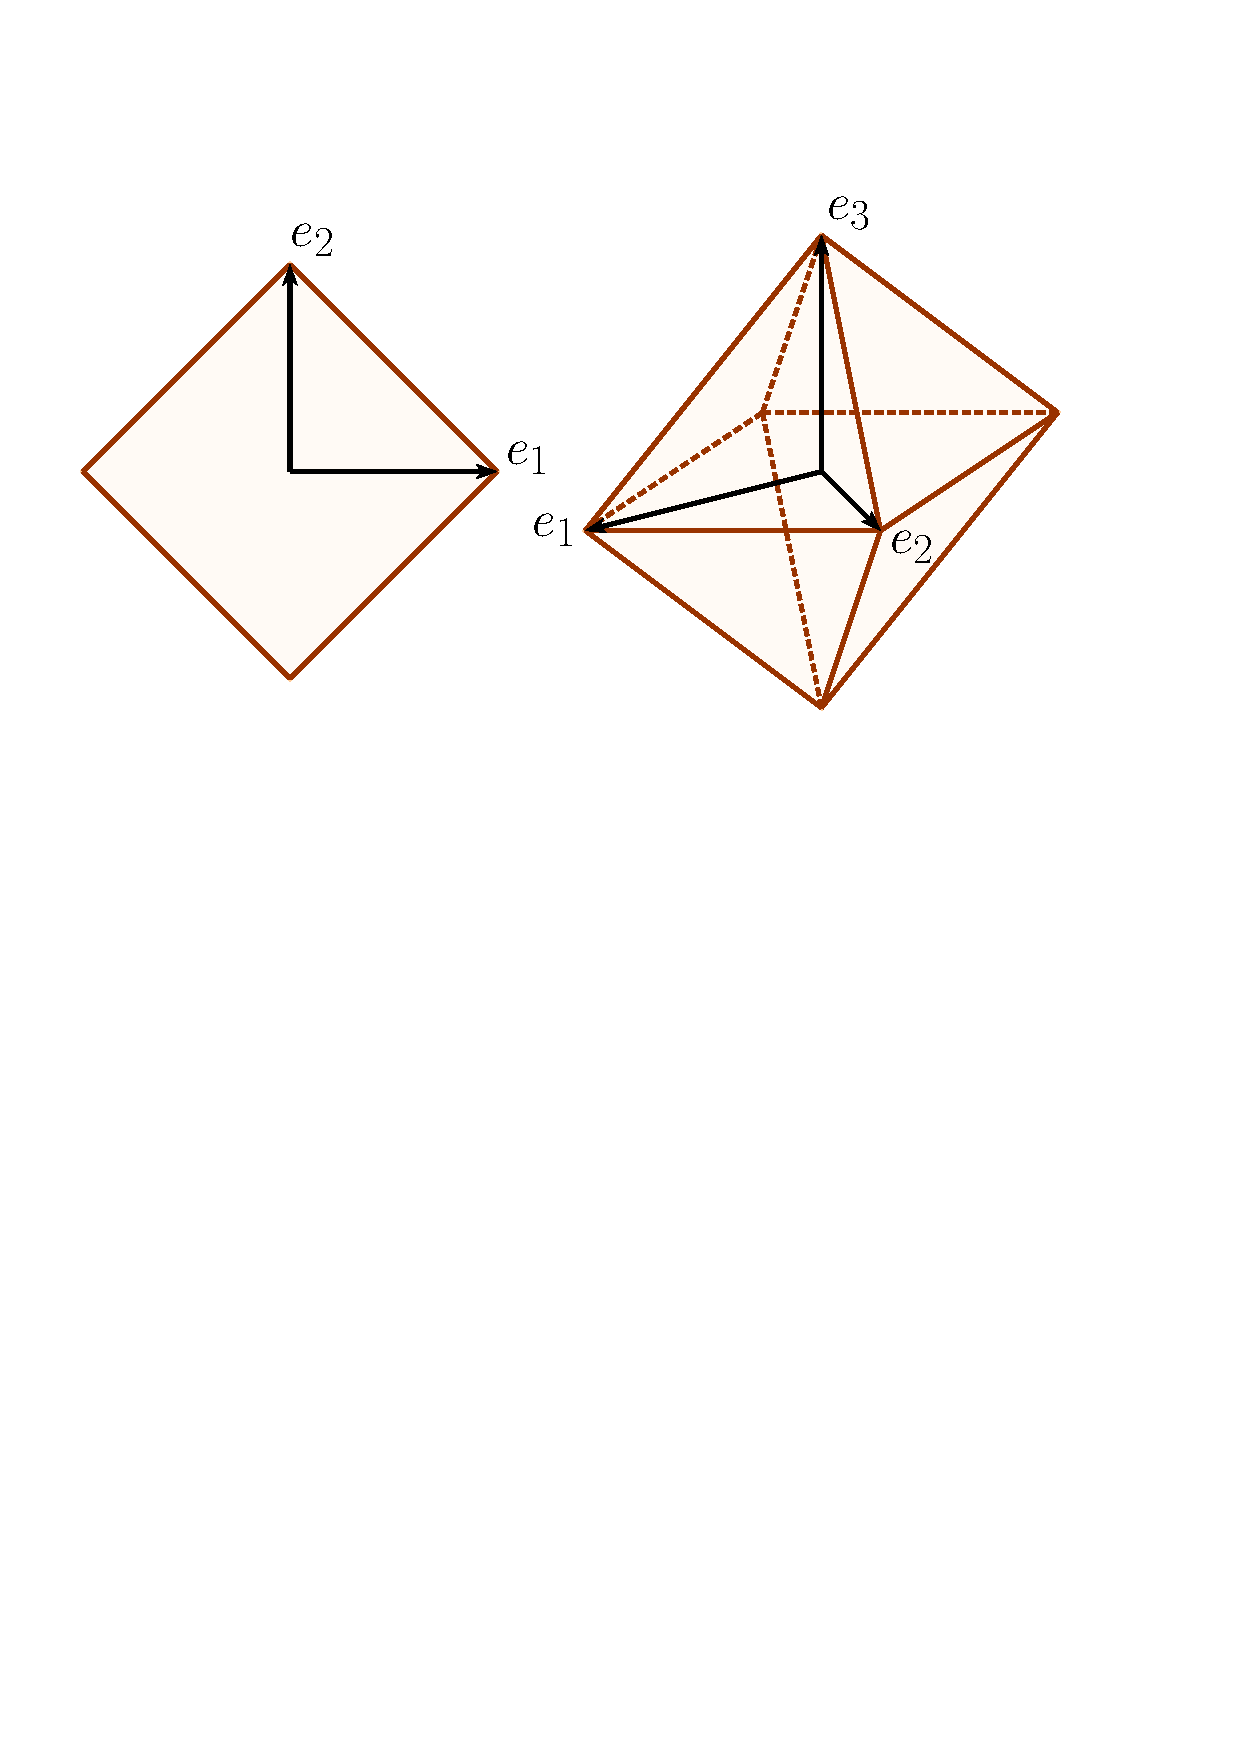
\includegraphics[scale=0.45]{pics/crosp.pdf}
			\caption{2- и 3-мерный кросс-политоп}
		\end{center}
	\end{figure}
\end{frame}

\begin{frame}{Введение}
	\framesubtitle{Постановка задачи}
	Рассматриваем
		$$F(H)=\vol(\crosp^n|H),$$
	где $\crosp^n|H$ -- ортогональная проекция кросс-политопа на $H\subset\RR^n$, $\dim H=k$.\\\pause
	\begin{task}
		\begin{equation*}
			\max_{\dim H=k}F(H)
		\end{equation*}
	\end{task}
\end{frame}

\begin{frame}{Введение}
	\framesubtitle{Известные оценки}
	\begin{thrm}[Барт, 1998]
		\begin{equation*}
			\vol(\crosp^n|H_k)\geqslant\left(\frac{k}{n}\right)^{k/2}\vol(\crosp^k)
		\end{equation*}\pause
	\end{thrm}
	\begin{thrm}[Барт, Наор, 2001]
		\begin{equation*}
			\cfrac{1}{\sqrt2}\vol(\crosp^{n-1})\leqslant\vol(\crosp^n|H_{n-1})\leqslant\vol(\crosp^{n-1})
		\end{equation*}
	\end{thrm}
\end{frame}

\begin{frame}{Введение}
	\framesubtitle{Двойственная задача}
	Напоминание: $K\subset\RR^n$,
		$$K^{\circ}=\{y\in\RR^n \ |\ \forall\ x\in K\ \langle x,y\rangle\leqslant 1\}$$
	\begin{eqnarray*}
		\crosp^n&\leftrightarrow&[-1,1]^n\\\pause
		K|H&\leftrightarrow&K^{\circ}\cap H\\\pause
		\vol(\crosp^n|H)&\leftrightarrow&\vol([-1,1]^n\cap H)\\
	\end{eqnarray*}
\end{frame}

\begin{frame}{Введение}
	\framesubtitle{Двойственная задача}
	\begin{thrm}[Ваалер, 1979]
		\begin{equation*}
			\vol([-1,1]^n\cap H)\geqslant\vol([-1,1]^k).
		\end{equation*}
	\end{thrm}\pause
	Иванов, 2018:
		\begin{equation*}
			\vol(\crosp^n|H)\leqslant\vol(\crosp^k),
		\end{equation*}
	доказано для случаев $k=2$, $k=3$.
\end{frame}

\begin{frame}{Введение}
	\framesubtitle{Основной результат}
	\begin{thrm}
		Пусть максимум объёма проекции $\vol(\crosp^n|H)$ достигается на 4-мерном подпространстве $H\subset\RR^n$. Тогда ненулевые проекции вершин кросс-политопа лежат на границе эллипсоида минимального объёма, содержащем $\crosp^n|H$, а их число не превосходит 20.
	\end{thrm}
\end{frame}

\begin{frame}{Эквивалентная формулировка}
	Пусть $H\subset\RR^n$ --- $k$-мерное подпространство,\\\pause
	$P$ --- оператор ортогональной проекции на $H$,\\\pause
	$\{e_i\}_1^n\subset\RR^n$ --- ОНБ, \pause $v_i=Pe_i$, $i=\overline{1,n}$,\pause
		$$\crosp^n|H=\co\{\pm v_i\}_1^n.$$
\end{frame}

\begin{frame}{Эквивалентная формулировка}
	\framesubtitle{Разложение единицы}
	Пусть $\{v_i\}_1^n\subset\RR^k$.\pause
	\begin{equation*}
		\{v_i\}_1^n\text{ --- проекция ОНБ}\Leftrightarrow\sum_1^n v_i\otimes v_i=I
	\end{equation*}\pause
	Набор векторов с таким свойством будем называть \textit{разложением единицы} в $\RR^k$.\\\pause
	Определим \textit{проекцию кросс-политопа, порождённую набором} $S=\{v_i\}_1^n\subset\RR^k$ как
		$$\crosp^n|S=\co\{\pm v_i\}_1^n.$$
\end{frame}

\begin{frame}{Эквивалентная формулировка}
	\framesubtitle{Разложение единицы}
	Глобальные экстремумы функций
	\begin{eqnarray*}
		F\colon\Gr(n,k)&\to&\RR\\
		H&\mapsto&\vol(\crosp^n|H)
	\end{eqnarray*}
	и
	\begin{eqnarray*}
		G\colon S\mapsto\vol(\crosp^n|S)
	\end{eqnarray*}
	совпадают.\\\pause
	Теперь максимизируем функцию $G(S)=\vol(\crosp^n|S)$.
\end{frame}

\begin{frame}{Метод возмущения разложения единицы}
	\begin{equation*}
		S\xrightarrow{T_1}\tilde{S}\xrightarrow{T_2}S'
	\end{equation*}\pause
	\begin{figure}[h!]
		\begin{center}
			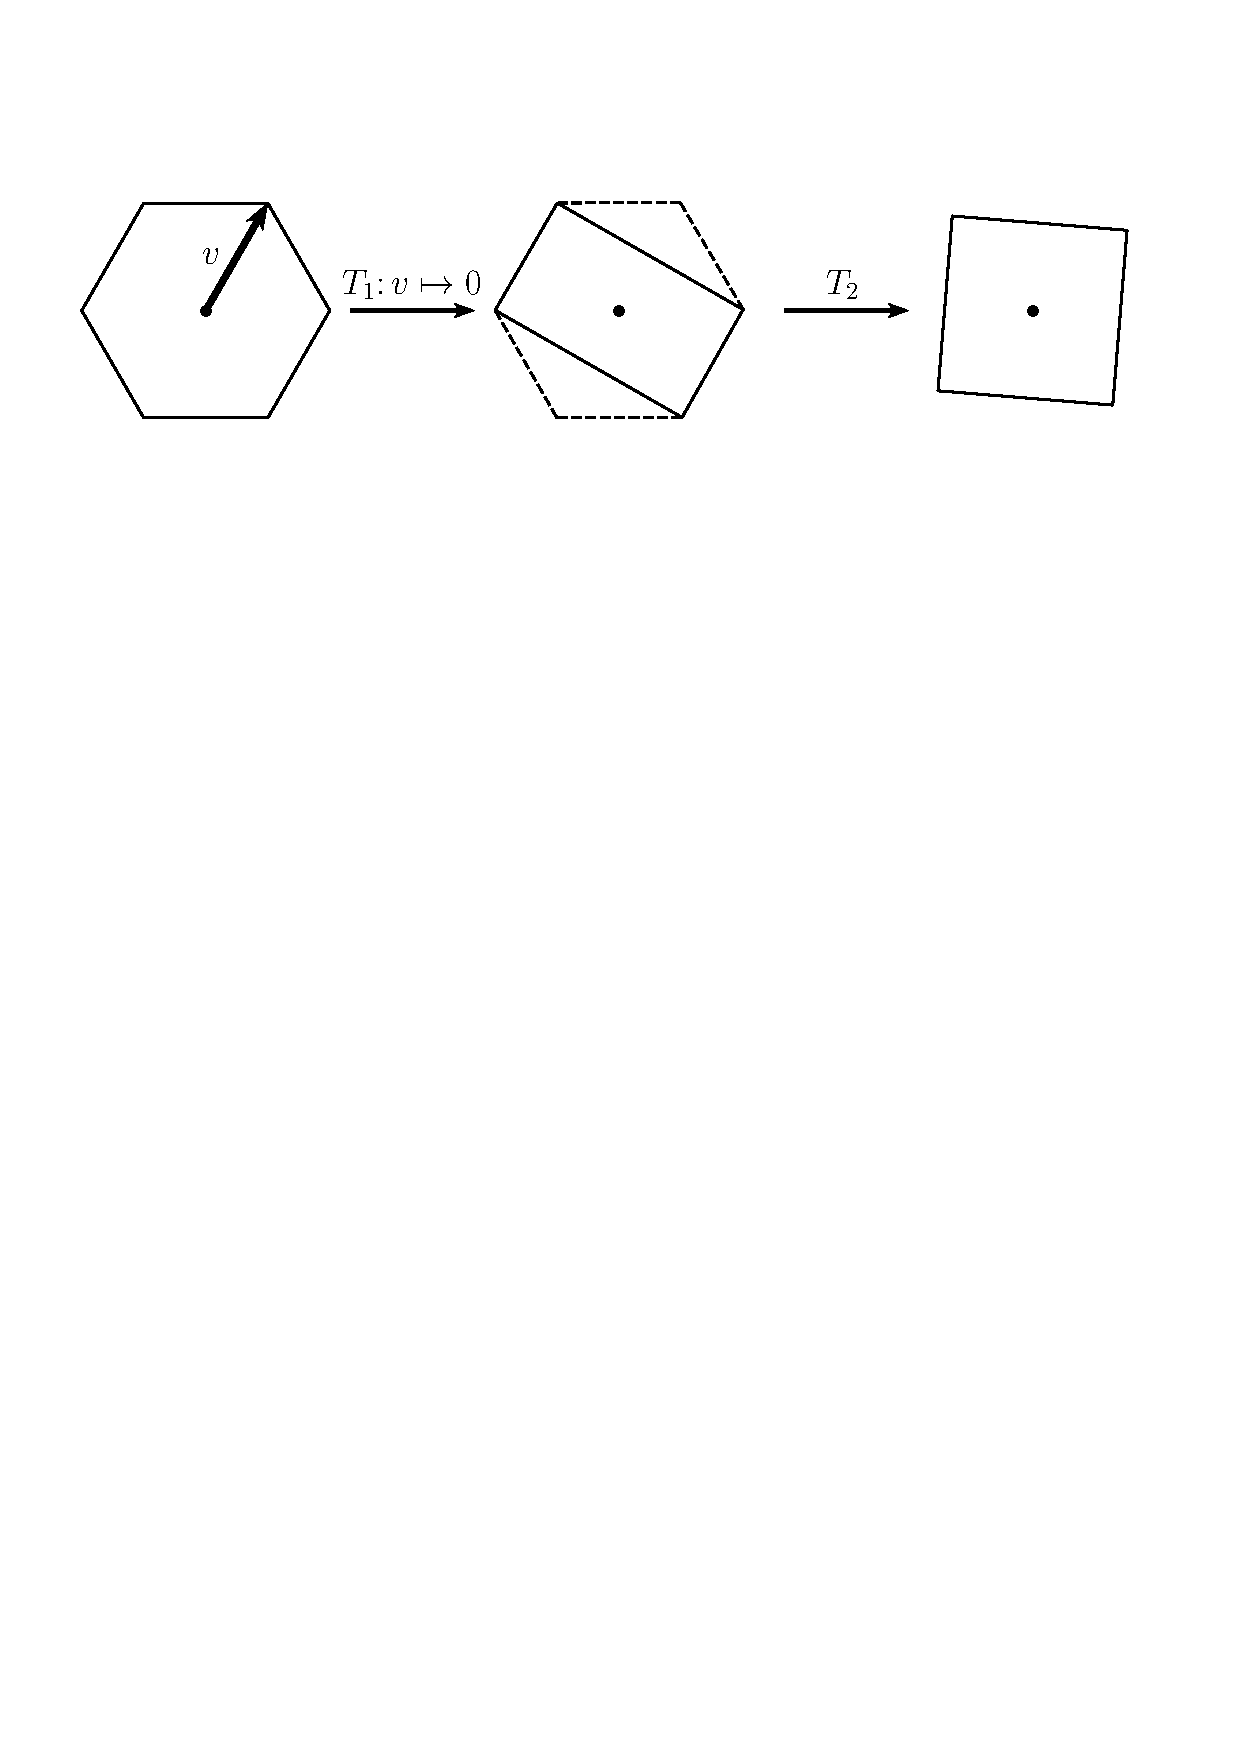
\includegraphics[scale=0.55]{pics/pertubation.pdf}
			\caption{Преобразование $T_1$ заменяет вектор $v$ на 0}
		\end{center}
	\end{figure}
\end{frame}

\begin{frame}{Метод возмущения разложения единицы}
	\framesubtitle{Критерий максмимальности объёма проекции}
	Для произвольного набора $\tilde{S}=\{u_i\}_1^n\subset\RR^k$ определим оператор
		\begin{equation*}
			A_{\tilde{S}}=\sum_1^n u_i\otimes u_i.
		\end{equation*}\pause
	Критерий:
		\begin{equation*}
			\frac{\vol(\crosp^n|\tilde{S})}{\vol(\crosp^n|S)}\leqslant\sqrt{\det A_{\tilde{S}}}.
		\end{equation*}\pause
		\begin{enumerate}
			\item слева: наглядные методы при выборе простого преобразования $T$;\pause
			\item справа: алгебраическая задача, можно решить точно или с нужной точностью.
		\end{enumerate}
\end{frame}

\begin{frame}{Эквивалентная формулировка}
	\begin{thrm}
		Пусть максимум функции $\vol(\crosp^n|S)$ при $k=4$ достигается на разложении единицы $S$ в $\RR^4$. Тогда ненулевые векторы набора $S$ лежат на границе эллипсоида минимального объёма, содержащего $\crosp^n|S$, а их число не превосходит 10.
	\end{thrm}
\end{frame}

\begin{frame}{Набросок доказательства}
	Эллипсоид Лёвнера $\low(K)$ выпуклого тела $K\subset\RR^k$ --- это эллипсоид минимального объёма, содержащий $K$.
	\begin{figure}[h!]
		\begin{center}
			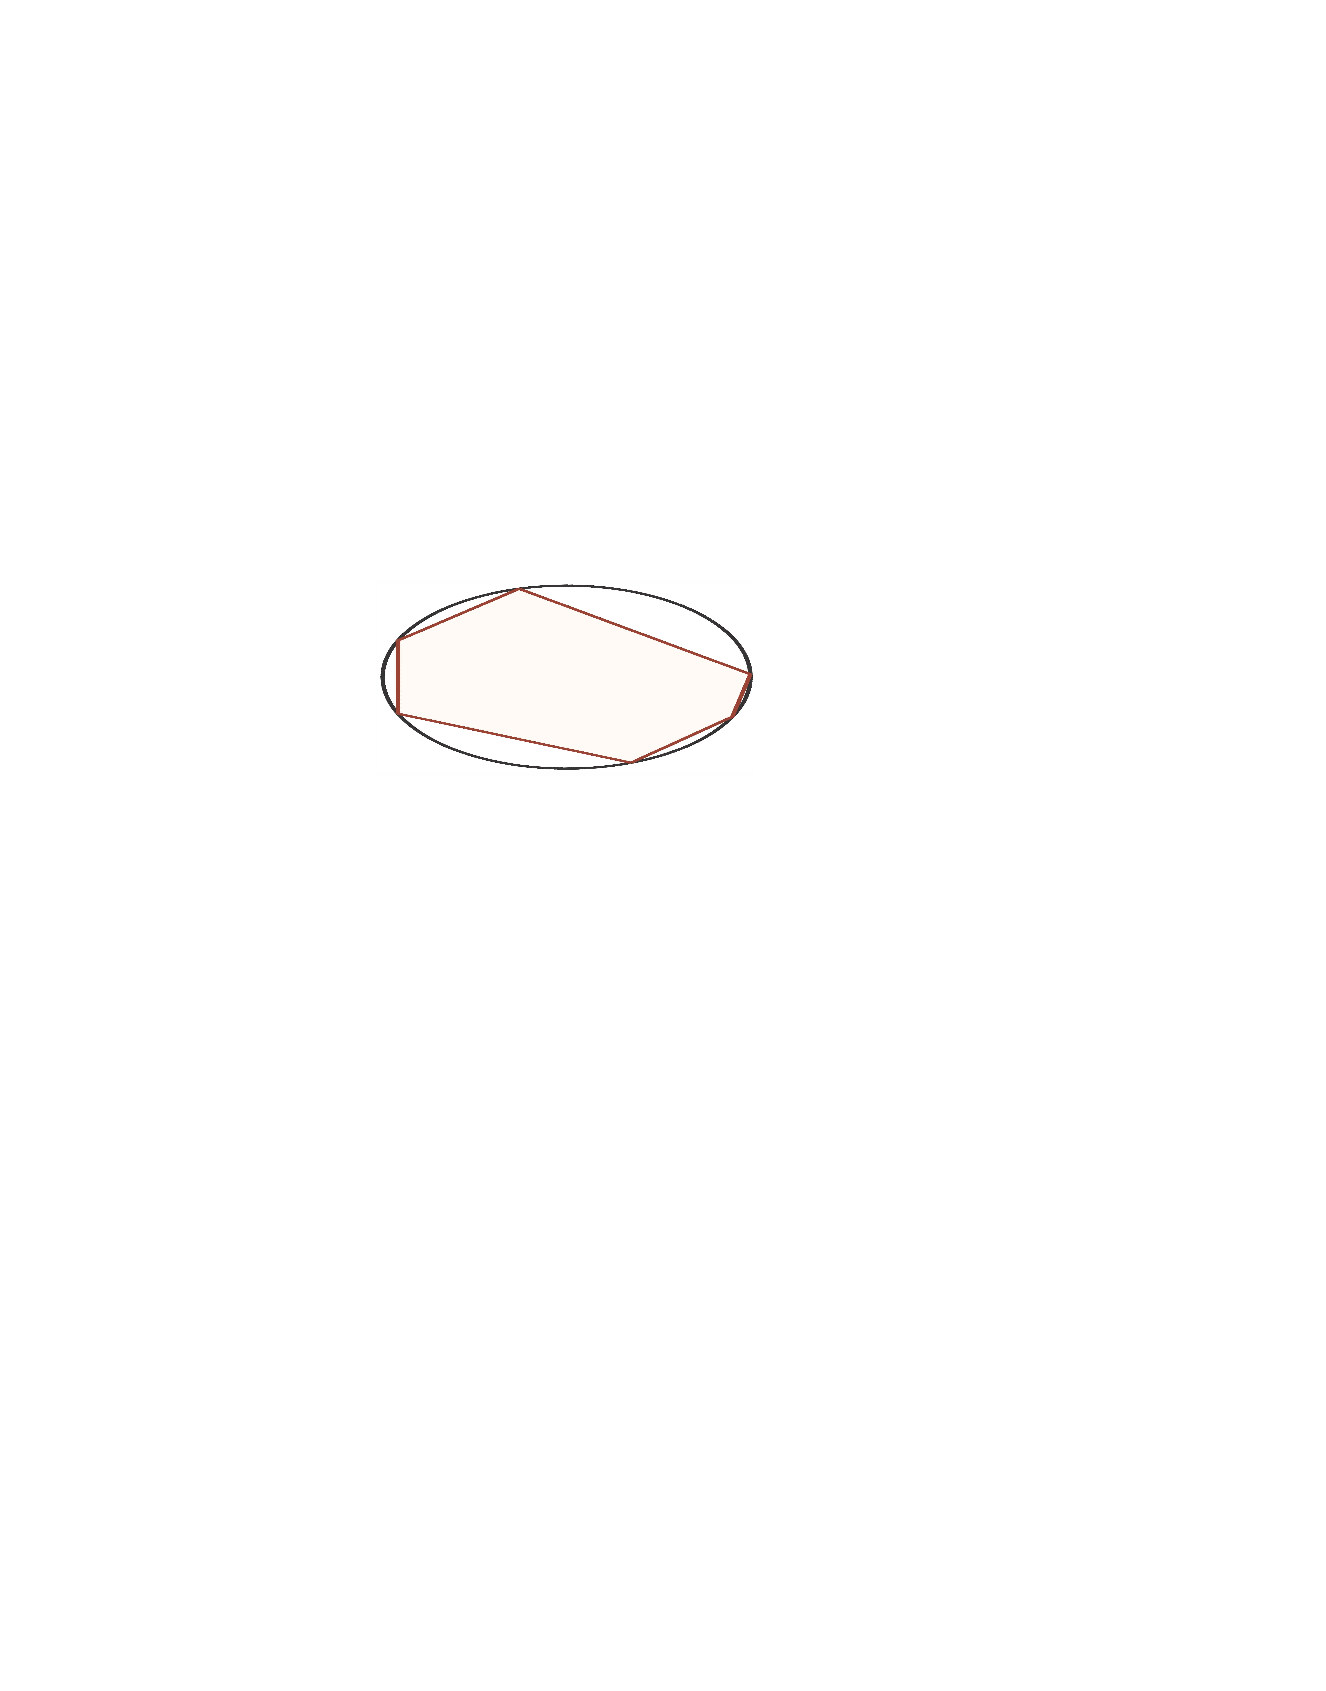
\includegraphics[scale=0.7]{pics/loewner.pdf}
			\caption{Эллипсоид Лёвнера многоугольника}
		\end{center}
	\end{figure}
\end{frame}

\begin{frame}{Набросок доказательства}
	\framesubtitle{Остаток вершины}
	\textit{Остаток вектора $v$ разложения единицы $S$} --- многогранник $\crosp^n|TS$, где $T\colon v\mapsto 0$.\pause
	\begin{figure}[h!]
		\begin{center}
			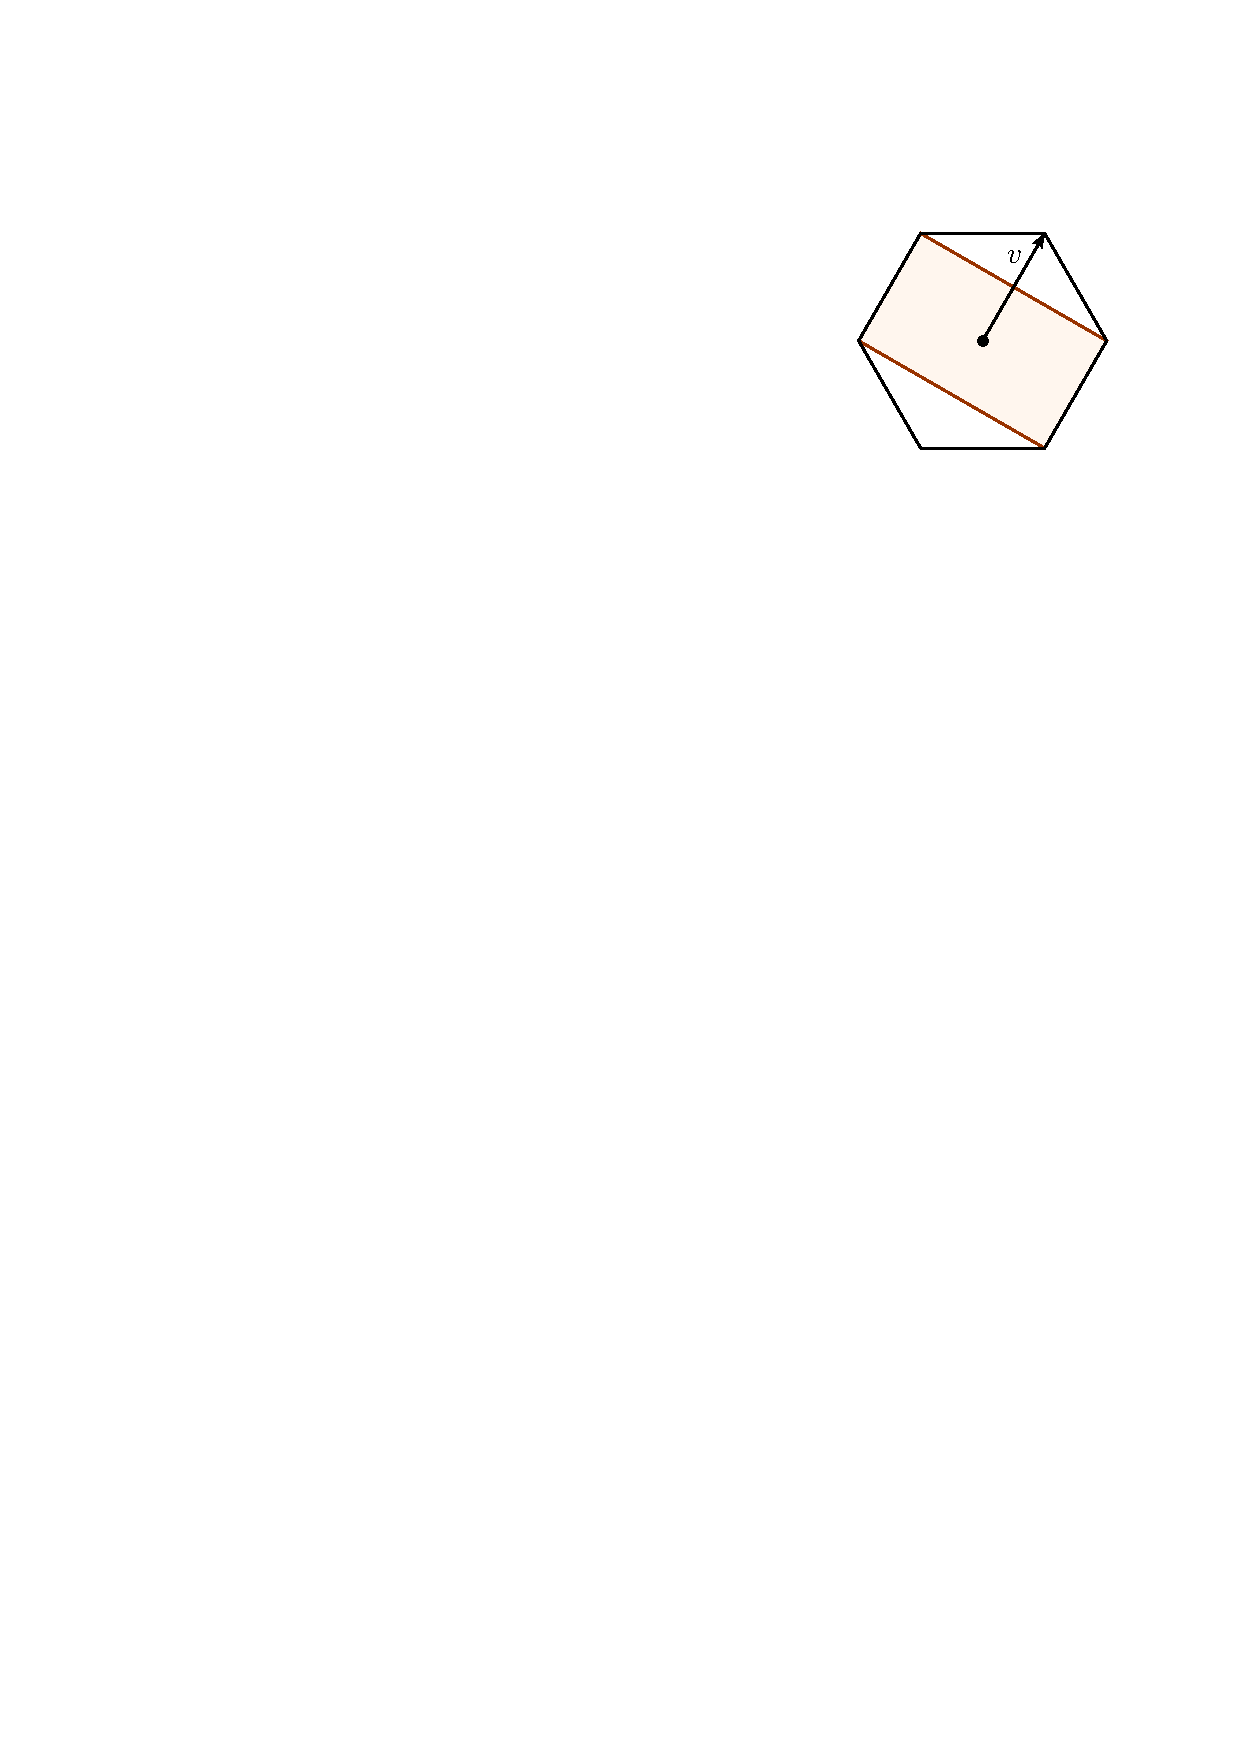
\includegraphics[scale=0.7]{pics/rest.pdf}
			\caption{Остаток вершины $v$ правильного шестиугольника}
		\end{center}
	\end{figure}
\end{frame}

\begin{frame}{Набросок доказательства}
	% Далее показываем, что ненулевые векторы разложения единицы $S$ в $\RR^4$ --- существенные вершины $\crosp^n|S$.\pause
	$v\in S$, $v\neq 0$.
	\begin{figure}[h!]
		\begin{center}
			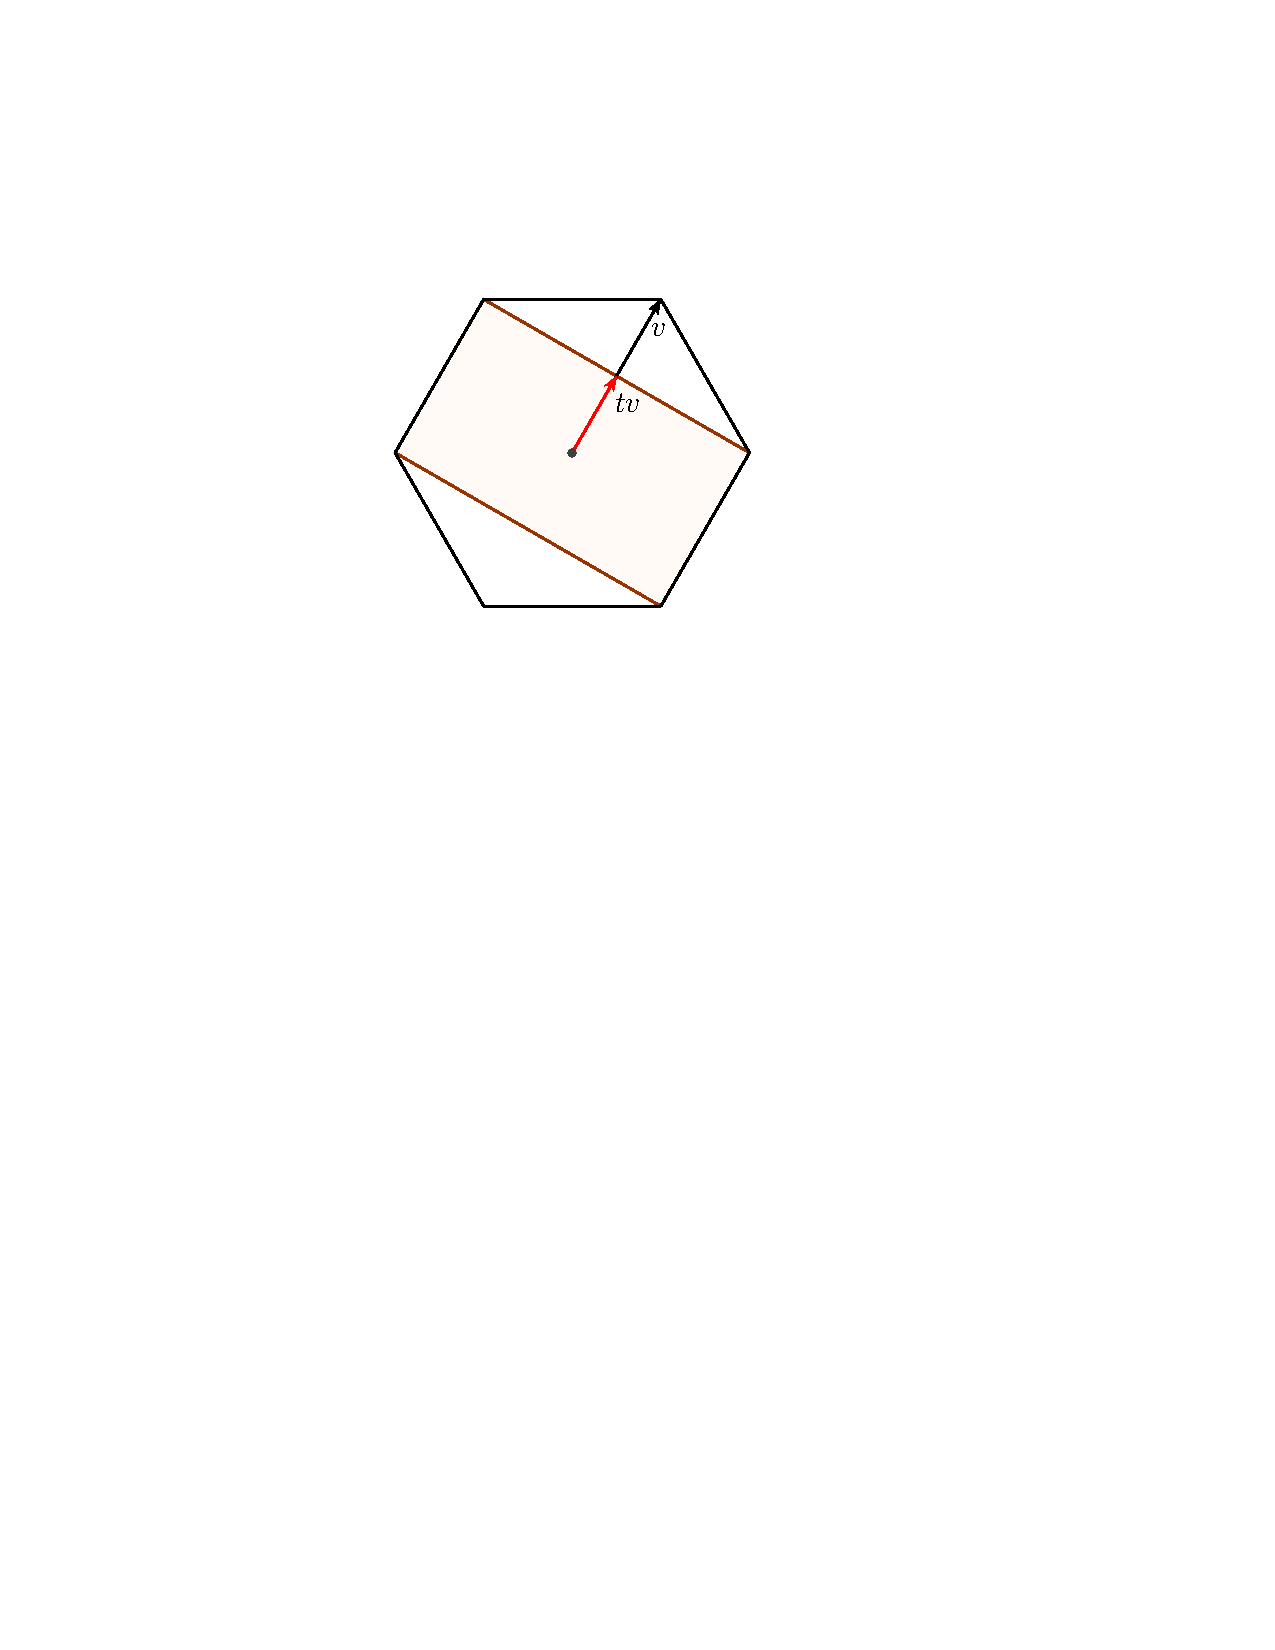
\includegraphics[scale=0.7]{pics/tv.pdf}
			\caption{$tv\in\partial\crosp^n|TS$}
		\end{center}
	\end{figure}\pause
	Применяя критерий, получаем
		$$0<t<1/2$$
	% Видно, что тогда $tv\in(1/2\ \low(M))$. Значит, $v$ --- существенная вершина, так как иначе $1/2\ \low(M)\subset R_M(v)$, что невозможно.
\end{frame}

\begin{frame}{Набросок доказательства}
	\framesubtitle{Фокус}
	Для эллипсоида Лёвнера центрально-симметричного выпуклого тела $K\subset\RR^4$ выполнено включение
		\begin{equation*}
			\frac{1}{2}\low(K)\subset K\subset\low(K)
		\end{equation*}\pause
	Значит, $tv\in\int(1/2\ \low(\crosp^n|S))$.\\\pause
	Далее $\low(\crosp^n|S)\neq\low(\crosp^n|TS)$.
\end{frame}

\begin{frame}{Набросок доказательства}
	\begin{lem}
		Существенные вершины выпуклого центрально-симметричного многогранника в $\RR^k$ лежат на границе его эллипсоида Лёвнера, а их число не превосходит $k(k+1)$.
	\end{lem}\pause
	Доказательство использует теорему Джона (1948) и её обратную часть, доказанную Боллом (1992).
\end{frame}

\begin{frame}{}
	\begin{center}
		Спасибо за внимание!\\
		Задавайте свои ответы.
	\end{center}
\end{frame}

\end{document}
